% !TeX spellcheck = pl_PL

\rozdzial

%%%%%%%%%%%%%%%%%%%%%%%%%%%%%%%%%%%%%%%%%%%%%%%%%%%%%%%%%%%%%%%%%%%%%%%
\section{Moduł graficzny}

Moduł graficzny jest najbardziej rozbudowanym elementem zaimplementowanym w~ramach tej pracy. Jego zadaniem jest przetwarzanie tekstu ze znacznikami formatującymi na obraz wideo. Przykładowy efekt działania modułu znajduje się na rysunku \ref{guiScreenExample}.

Najważniejszą cechą wyróżniającą ten moduł od innych rozwiązań jest to, że przetwarzanie tekstu na grafikę odbywa się natychmiastowo przy generowaniu sygnału na wyjście wideo. Taka metoda nie wymaga buforowania całej zawartości ekranu w pamięci przez co zużycie RAM jest niewielkie. Minimalny rozmiar pamięci wystarczający do wyświetlenia interfejsu użytkownika to 2 BRAM'y układu FPGA, czyli 36 kbit (4,5 KB) lub 3 BRAM'y (6,75 KB), gdy moduł ma obsługiwać kursor myszy i obrazy rastrowe. Dodatkowo można uzyskać duże rozdzielczości ekranu (nawet FullHD - 1920x1080 pikseli), bez konieczności zwiększania ilości pamięci.

\begin{figure}[htb]
	\centering
	\obrazpng{0 0 1024 625}{13cm}{obrazki/guiPhoto.jpeg}
	\caption{Przykładowe zdjęcie ekranu wyświetlającego wyjście modułu graficznego.}
	\label{guiScreenExample}
\end{figure}


Moduł nadal oferuje możliwości pozwalające na stworzenie przyjaznej dla użytkownika grafiki mimo tak niewielkich wymagań co do rozmiaru pamięci. Dodatkowo na pozytywne wrażenia użytkownika może wpłynąć fakt, że zastosowane tu wygładzanie optyczne czcionek z dwoma odcieniami pośrednimi. Porównując wynik działania modułu z prostymi rozwiązaniami przedstawionymi w rozdziale \ref{Proste_rozwiązania} można stwierdzić, że grafika generowana przez ten moduł jest bardziej przyjazna użytkownikowi.


%%%%%%%%%%%%%%%%%%%%%%%%%%%%%%%%%%%%%%%%%%%%%%%%%%%%%%%%%%%%%%%%%%%%%%%
\subsection{Metoda renderowania grafiki}
\label{MetodaRenderowaniaGrafiki}

Moduł przetwarza tekst ze znacznikami formatującymi na sygnał wideo. Tekst ten znajduje się w pamięci BRAM. Procesor PicoBlaze ma pełen dostęp do tej pamięci, więc może w pełni kontrolować grafikę wyświetlaną na ekranie.

Tekst ze znacznikami formatującymi może posiadać następujące elementy:
\begin{itemize}
	\item Kody ASCII - wartości od 32 do 126
	\item Znaki niestandardowe, np. polskie znaki, symbole graficzne - wartości od 0 do 31
	\item Znaczniki do obsługi kolorów:
	\begin{itemize}
		\item Modyfikacja palety 16 kolorów
		\item Wybranie koloru znaku lub tła z palety kolorów
	\end{itemize}
	\item Znaczniki do obsługi pozycji na ekranie:
	\begin{itemize}
		\item Tabulacja do wybranej kolumny
		\item Koniec wiersza oraz określenie jego wysokości
		\item Odstępy o niestandardowej szerokości
	\end{itemize}
	\item Znaczniki pozwalające na przejście do innej pozycji w tekście, np. inne okno
	\item Znaczniki obsługi myszy
	\begin{itemize}
		\item Zmiana aktualnego położenia kursora myszy
		\item Zmiana wyglądu kursora myszy
		\item Rozpoczęcie i zakończenie kontrolki używane do określenia nad czym znajduje się aktualnie kursor myszy
	\end{itemize}
	\item Znaczniki do obsługi bitmap rastrowych
\end{itemize}

Powyższa lista może wydawać się niewielka, jednak odpowiednie operowanie na znacznikach tabulacji, nowego wiersza i zmiany kolorów pozwana na generowanie bardziej zaawansowanych elementów, m.im. ramki, tabele, okna, przyciski, listy, pola tekstowe.

Bezpośrednie zapisywanie kodów liczbowych znaczników w tekście mogłoby być bardzo uciążliwe, dlatego został wykonany skrypt konwertujący tekst w przyjaznej dla użytkownika formie na kod źródłowy Verilog. Tak wygenerowany plik można dodać do reszty projektu. Przykładowy tekst wejściowy dla tego skryptu znajduje się na rysunku~\ref{ftExample}. Ten przykład pokazuje jak wyświetlić na ekranie proste okienko z~wiadomością oraz przyciskami ,,OK'' i ,,Cancel''.

\begin{figure}[htb]	
	\centering
	\setlength{\fboxsep}{0pt}
	\setlength{\fboxrule}{0.5pt}
	\fbox{\obrazpng{0 0 1024 625}{16cm}{obrazki/ftExample.png}}
	\caption{Przykładowy tekst ze znacznikami formatującymi}
	\label{ftExample}
\end{figure}

Tak przygotowany kod będzie dostępny dla programisty z poziomu procesora PicoBlaze. W celu sterowania zawartością ekranu wystarczy zmieniać odpowiednie znaczniki i litery w tym kodzie. To zadanie spełnia biblioteka graficzna. Jest ona opisana w rozdziale~\ref{guilib_section}.

Tworzenie obrazu na ekranie odbywa się przez pobieranie kolejnych kodów (znaczników lub liter) z pamięci tekstu i renderowaniu ich na ekranie. Odbywa się to ,,w~locie'', czyli kolor piksela obrazu wyznaczany jest w momencie, gdy zostaje on wysłany na wyjście wideo -- nie jest używana żadna dodatkowa pamięć w tym miejscu. Istnieje pewna wada takiego rozwiązania: kody, które nie są literami również generują pewniej szerokości pusty znak, ponieważ potrzeba co najmniej jeden takt zegara, aby je zinterpretować i wykonać. Rysunek \ref{renderExample} przedstawia przykład, gdzie bezpośrednio po sobie następują dwa znaczniki zmiany koloru tła, co generuje pionową linię o szerokości jednego piksela. Ta technika jest używana jako jeden ze sposobów tworzenia ramek lub tabel.

\begin{figure}[htb]	
	\centering
	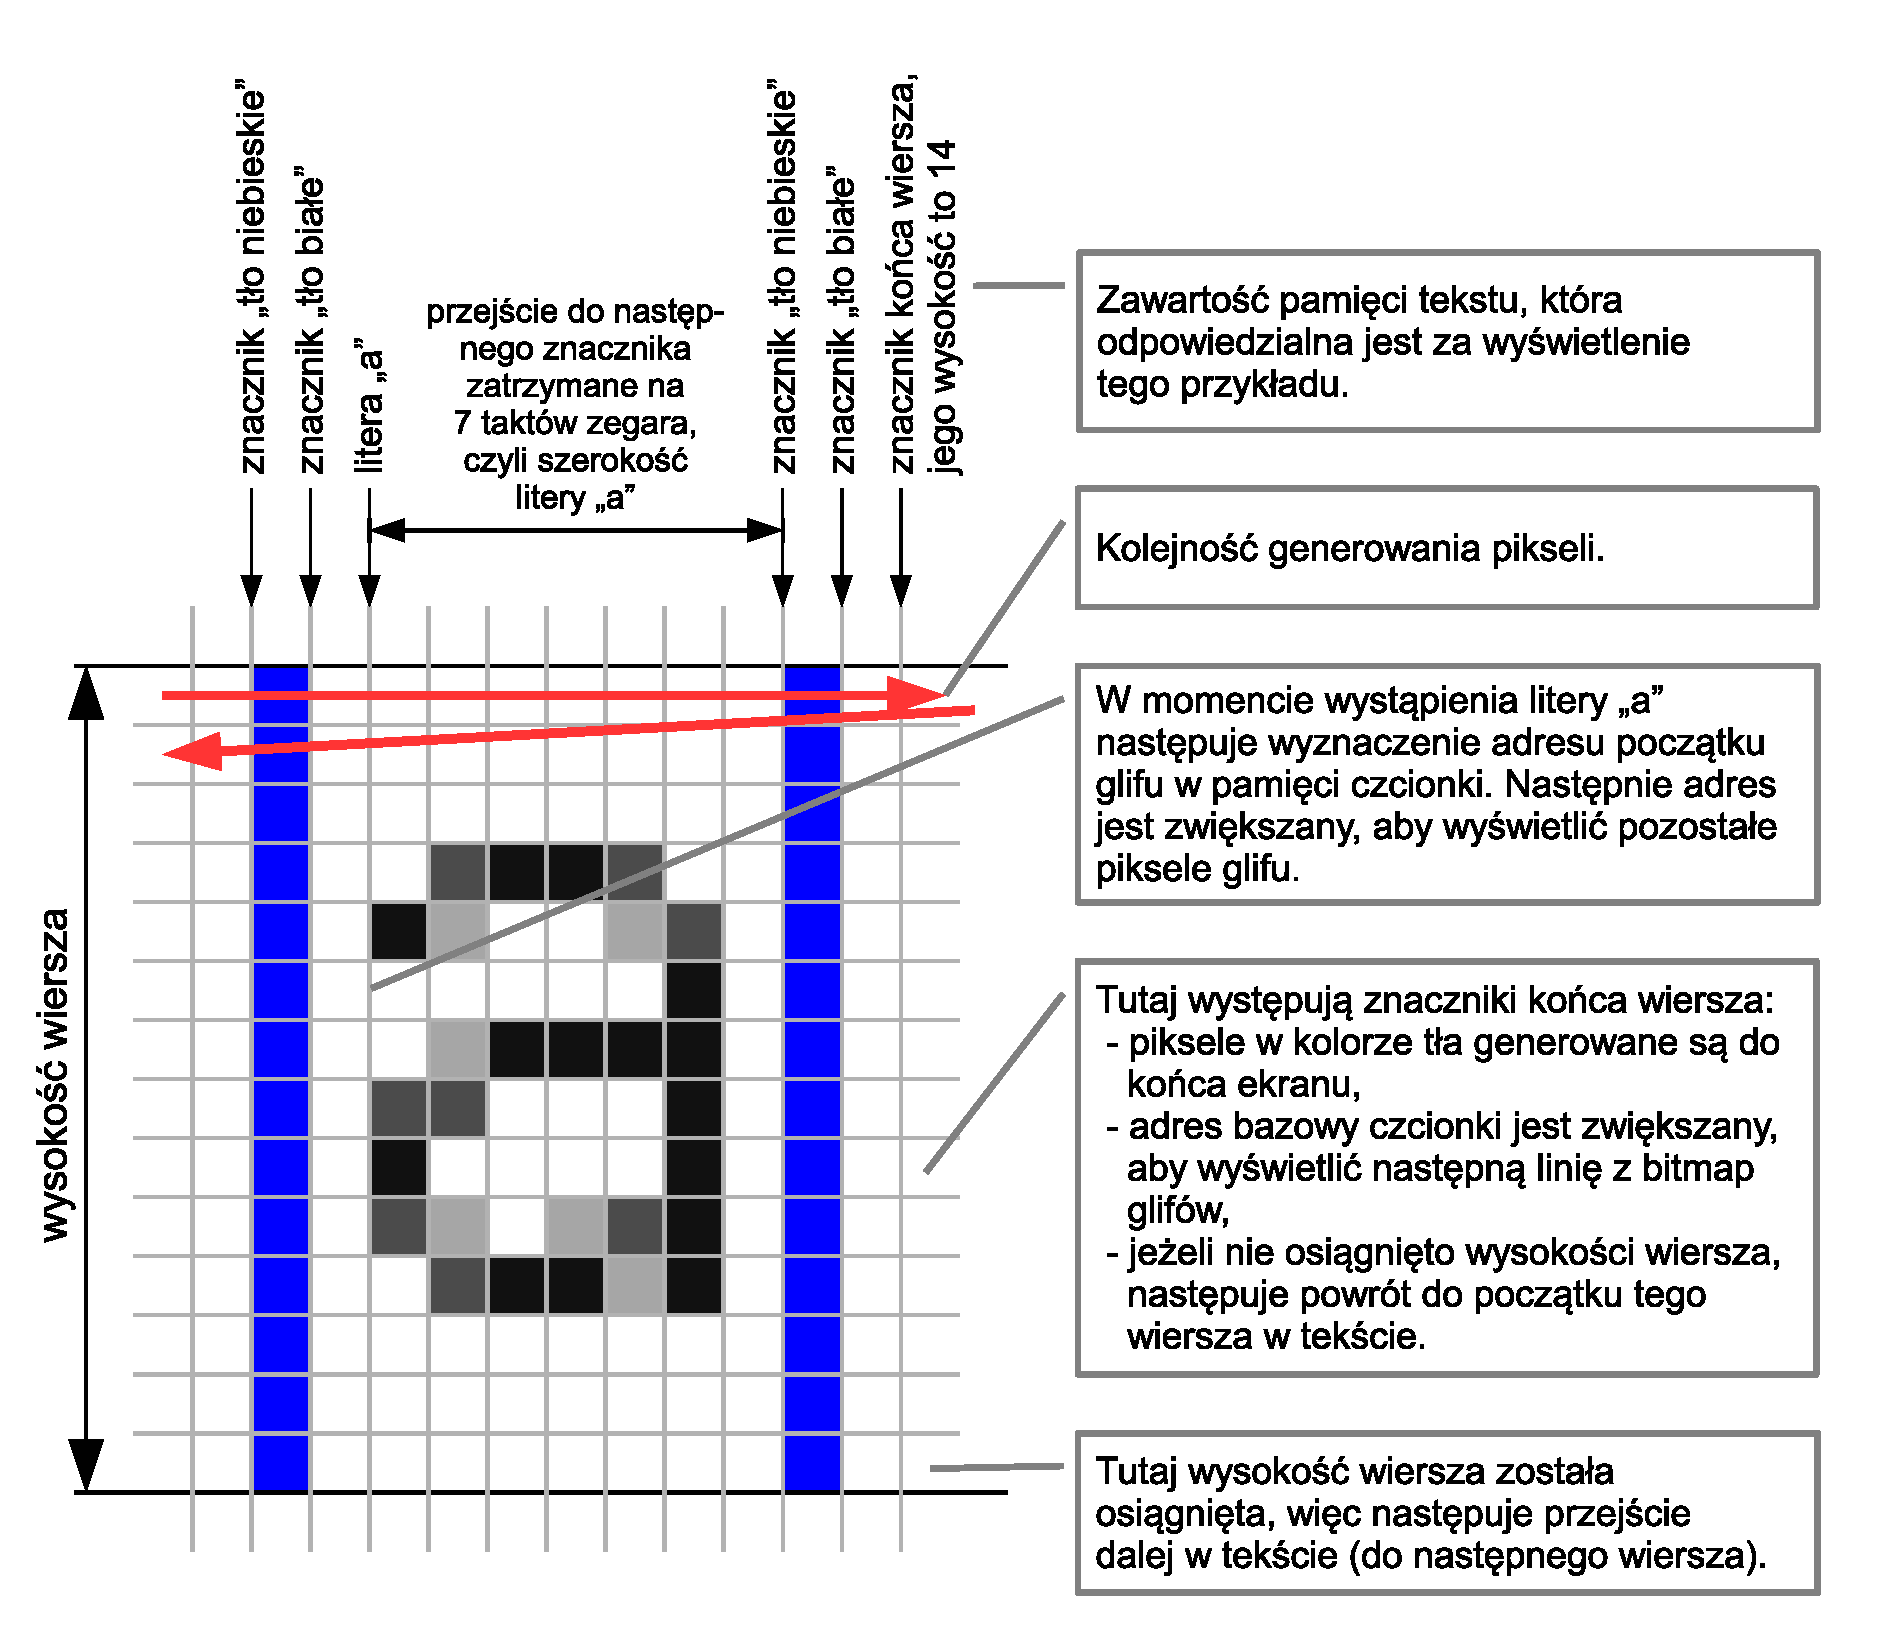
\includegraphics[width=14cm]{obrazki/renderExample.eps}
	\caption{ Przykład renderowania litery ,,a'' otoczonej dwoma niebieskimi pionowymi liniami. }
	\label{renderExample}
\end{figure}

Każdy kod jest przetwarzany na adres w pamięci czcionek, gdzie znajdują się informacje o danym znaku. Po odczytaniu tych informacji znana jest szerokość znaku oraz adres, gdzie znajduje się obraz bitmapowy glifu reprezentującego ten znak. W~kolejnych taktach zegara piksele z tej bitmapy wędrują na wyjście wideo, aż zadana szerokość zostanie osiągnięta. Następnie pobierany jest kolejny kod i przetwarzany w ten sam sposób. Znaczniki oprócz tego, że mają specjalne działanie, również generują znak, ale jest on pusty -- wszystkie piksele mają kolor tła.

W momencie dojścia do znacznika końca wiersza następuje skok warunkowy w pamięci tekstu. Jeżeli liczba linii obrazu w tym wierszu nie jest taka, jak podaje znacznik, to następuje powrót do początku tego wiersza w tekście, aby wyświetlić następną linię obrazu należącą do wiersza. Rysunek \ref{renderExample} pokazuje to na przykładzie.

Pamięć czcionki musi zawierać dane przystosowane do tej metody renderowania, dlatego powstało narzędzie, które przetwarza dowolną czcionkę obsługiwaną przez system operacyjny komputera na kod źródłowy Verilog. Wygenerowany plik zwiera blok pamięci z~gotową zawartością, który może zostać dołączony do modułu. Dzięki temu zmiana wyglądu czcionki jest bardzo prosta, a liczba dostępnych krojów jest niemal nie ograniczona.


%%%%%%%%%%%%%%%%%%%%%%%%%%%%%%%%%%%%%%%%%%%%%%%%%%%%%%%%%%%%%%%%%%%%%%%
\subsection{Wyświetlanie kursora myszy i obrazów rastrowych}

Opcjonalnie moduł może zostać wyposażony w~możliwość wyświetlania grafiki rastrowej. Metoda opisana w rozdziale \ref{MetodaRenderowaniaGrafiki} nie jest wystarczająca do tego celu.


Ważnym elementem interfejsu graficznego jest kursor myszy, który jest bitmapą posiadającą przeźroczyste piksele nałożoną na pozostałą część grafiki. Pamięć tekstu może zawierać znaczniki, które powodują ustawienie współrzędnych kursora myszy. Procesor może modyfikować wartości w tych znacznikach w celu przesuwania kursora. Istnieją znaczniki, które informują moduł która aktualnie kontrolka jest generowana. Jeżeli kursor znajdzie się na obszarze danej kontrolki, to następuje zapis unikalnego identyfikatora kontrolki do rejestru, który jest dostępny z poziomu procesora. To pozwala uprościć kod programu i ilość pamięci zajmowanej w procesorze, ponieważ program nie musi pamiętać współrzędnych każdej kontrolki.


Jeżeli generowany piksel znajduje się w obszarze zajmowanym przez kursor myszy, to następuje odczytanie kolejnych pikseli z pamięci kursorów. Istnieje możliwość zmiany początkowego adresu piksela w celu ustawienia kształtu kursora. Aktualnie zostały wykonane trzy kształty: strzałka, rączka i klepsydra. Istnieje możliwość zdefiniowania do 8 kształtów kursorów o wymiarach do 24 na 24 piksele. Bitmapa zawiera cztery kolory: czarny, biały, szary i przeźroczysty. Piksel zostanie podany na wyjście wideo, jeżeli kolor jest inny niż przeźroczysty. W przeciwnym wypadku zostanie użyty piksel pod kursorem.


Wyświetlanie obrazów rastrowych wykonywane jest przez znaczniki w pamięci tekstu. Istnieją dwa znaczniki do kontroli bitmap. Pierwszy ustala adres pierwszego piksela w~pamięci bitmap, która jest współdzielona z pamięcią kursorów. Drugi znacznik powoduje rozpoczęcie i zakończenie podawania pikseli z bitmapy na wyjście wideo.


%%%%%%%%%%%%%%%%%%%%%%%%%%%%%%%%%%%%%%%%%%%%%%%%%%%%%%%%%%%%%%%%%%%%%%%
\subsection{Struktura modułu}


Struktura modułu graficznego przedstawiona jest na rysunku \ref{render_flow}. Cały moduł został podzielony na mniejsze elementy spełniające poszczególne zadania. Taka struktura pozwala na lepsze zarządzanie kodem źródłowym, zrozumieniem działania i~zależności, a także łatwiejszy rozwój.

Sercem modułu jest dekoder tekstu ze znacznikami formatującymi ,,TextDecoder'', który odpowiedzialny jest za odczyt danych z pamięci tekstu, ich interpretację i~sterowanie dalszymi elementami. Jego działanie w pewnym stopniu jest zbliżone do działania dekodera instrukcji w procesorach. Efektem dekodowania są informacje o~kursorze myszy, wyświetlanej bitmapie, kolorze tła i czcionki oraz kodzie znaku, który ma zostać wyświetlony następnie.

Pamięć czcionki używana w trybie ROM ,,FontMemory'' zawiera informacje o glifie skojarzonym z tym kodem. Kolejny element w tej ścieżce ,,GlyphAddrGen'' generuje adres wskazujący na bitmapę glifu. Informuje również dekoder tekstu o przejściu do następnego kodu, gdy cała szerokość glifu zostanie wyświetlona. Adres glifu jest przekształcany na adres piksela glifu przez kolejny element ,,FontAddrGen''. Następnie piksel o tym adresie jest odczytywany z 2-bitowej bitmapy zawartej w drugiej części pamięci czcionek ,,FontMemory''.

Mikser kolorów ,,ColorMixer'' jest odpowiedzialny za generację odpowiedniego koloru wyjściowego na podstawie koloru tła, koloru czcionki i jasności aktualnego piksela glifu. Dalej trafia do multipleksera wybierającego aktualne źródło pikseli ,,PixelMux''. Najlepszym rozwiązaniem jest generowanie średniej ważonej koloru tła i czcionki ze współczynnikiem pochodzącym z glifu, jednak takie rozwiązanie nie jest optymalne pod względem ilości zasobów. Dla uproszczenia zostało zastosowane inne mapowanie kolorów przedstawione w tabeli \ref{tab:colorMixer}. Tak wyświetlona czcionka nadal daje dobre wrażenie wizualne.

\begin{table}[h]
	\begin{center}
		{\footnotesize
			\begin{tabular}{|r|r|r|}
				\hline \textbf{Piksel glifu} & \textbf{Waga koloru czcionki} & \textbf{Waga koloru tła} \\
				\hline 0 & 100\% & 0\% \\
				\hline 1 & 50\% & 50\% \\
				\hline 2 & 25\% & 75\% \\
				\hline 3 & 0\% & 100\% \\
				\hline 
			\end{tabular}}
			\caption{ Wagi kolorów czcionki i tła dla różnych wartości piksela glifu. }
			\label{tab:colorMixer}
		\end{center}
	\end{table}


\begin{sidewaysfigure}[p]
	\centering
	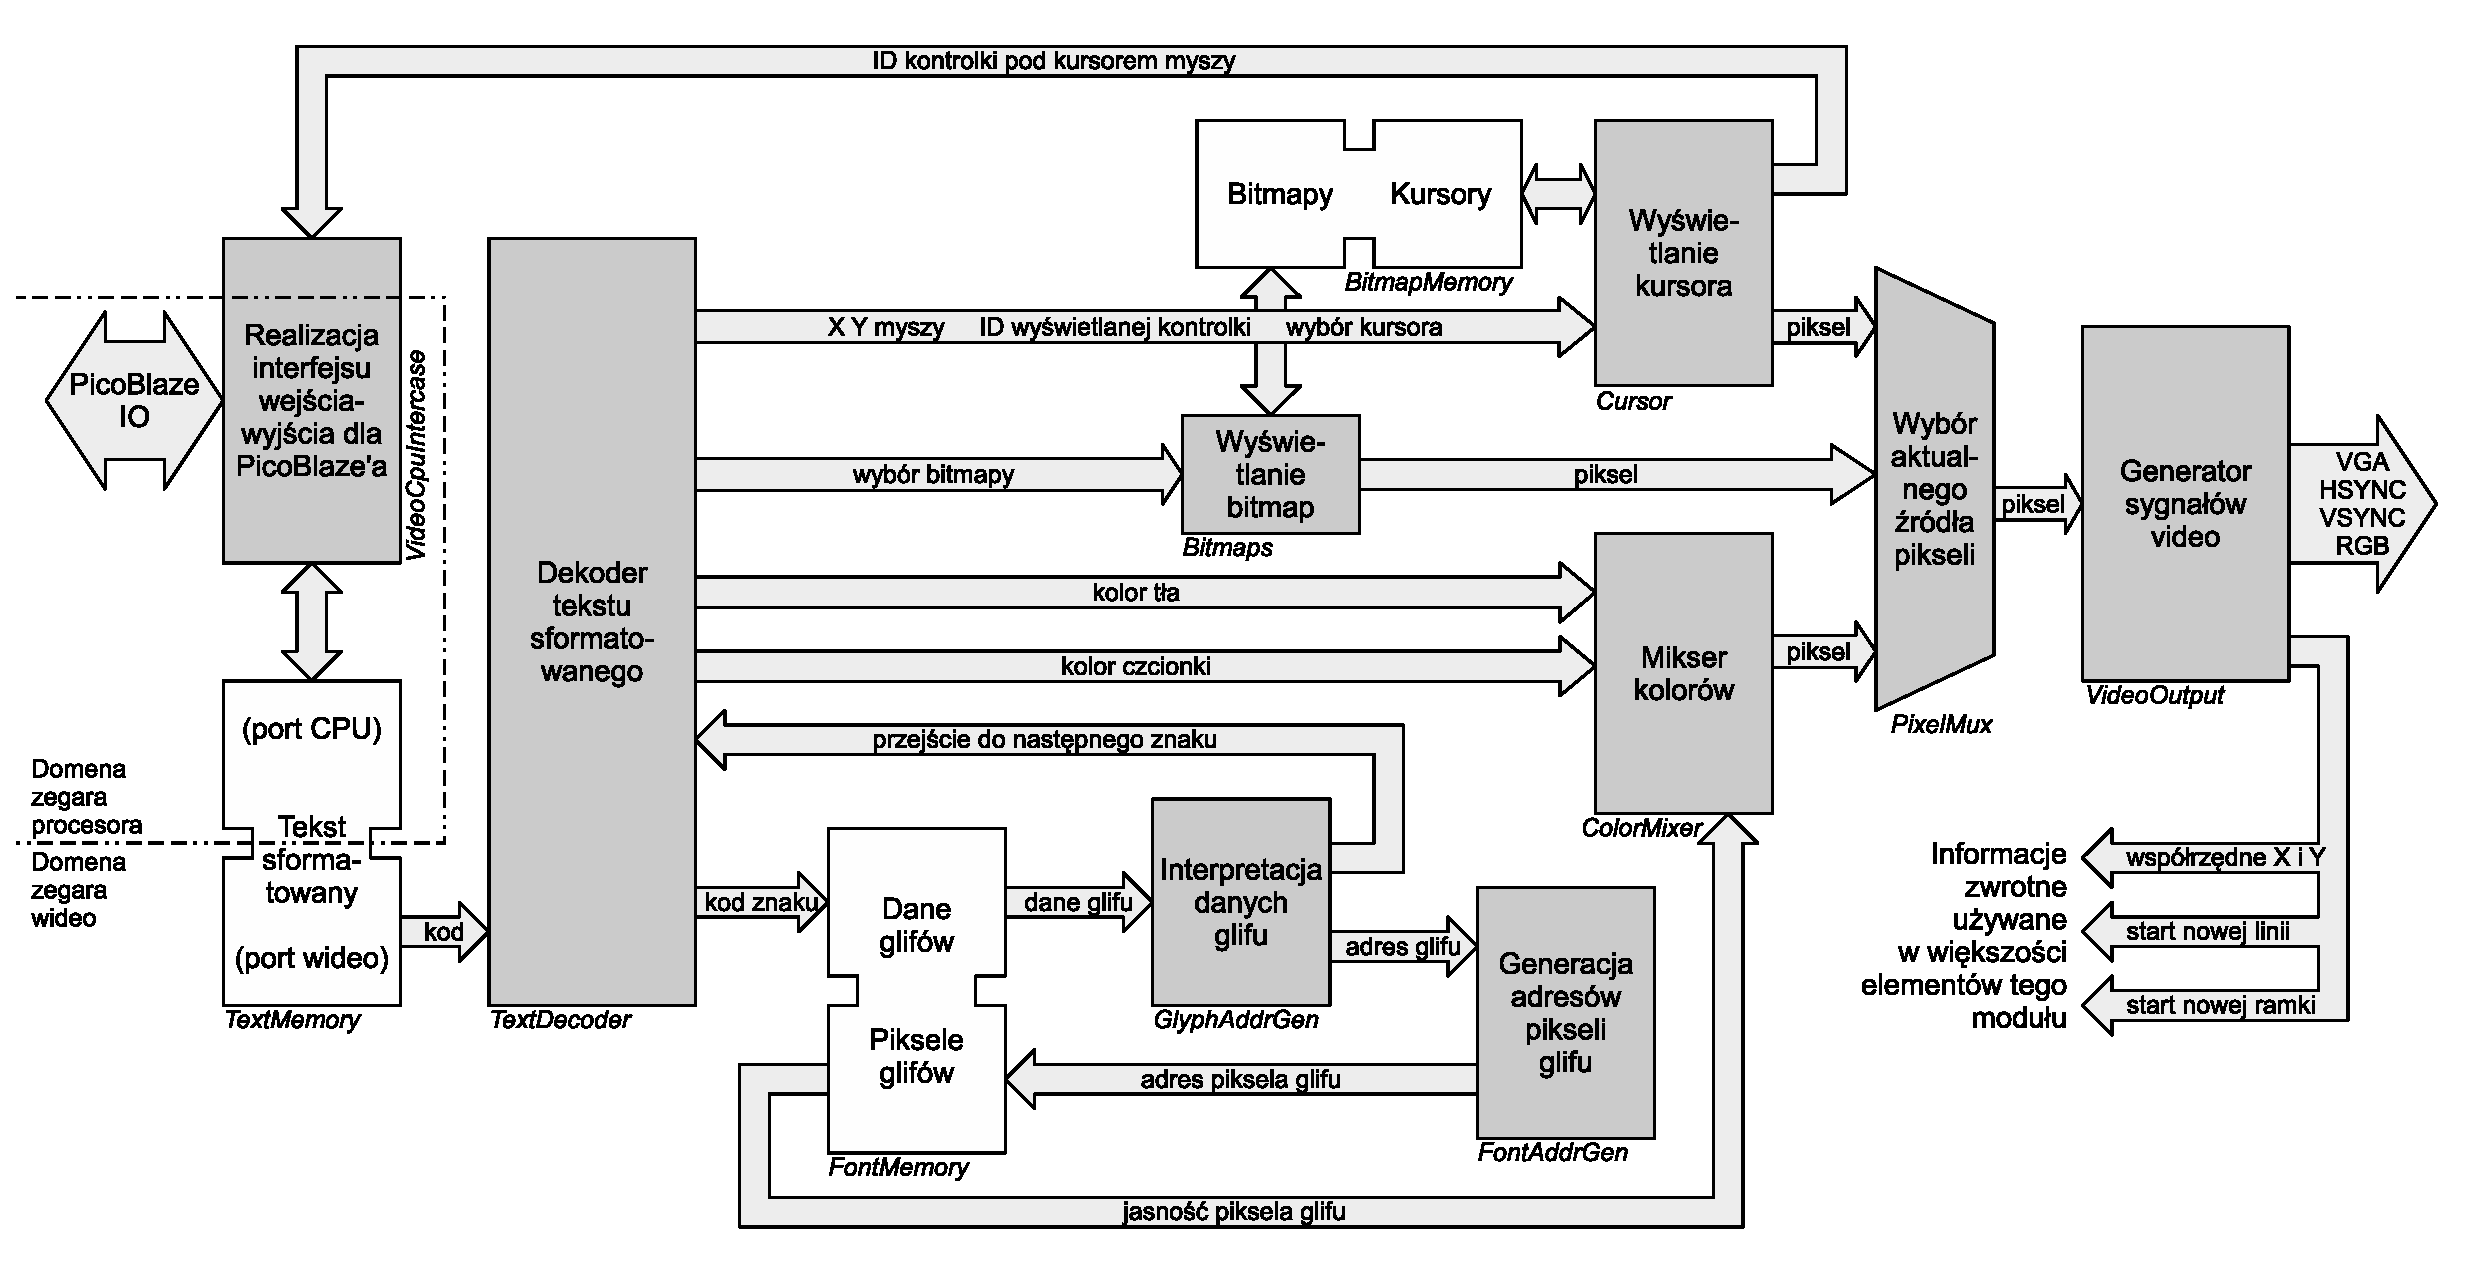
\includegraphics[width=22cm]{obrazki/render_flow.eps}
	\caption{ Uproszczony schemat modułu graficznego. }
	\label{render_flow}
\end{sidewaysfigure}

\clearpage

Oprócz tekstu możliwe jest również wyświetlanie bitmap. Bitmapy zapisane są w~pamięci ,,BitmapMemory''. Znajdują się tam dwa rodzaje bitmap. Jeden rodzaj posiada 9 bitów na piksel i jest wyświetlany przez element ,,Bitmaps'' na podstawie danych z dekodera. Drugi rodzaj bitmapy jest używany do wyświetlania kursora myszy przez element ,,Cursor'' również na postawie danych z dekodera. Dodatkowo jest wysyłana wartość identyfikatora kontrolki, nad którą aktualnie znajduje się kursor myszy, do interfejsu dla procesora.

Generator sygnałów wideo ,,VideoOutput'' tworzy i wysyła sygnały na wyjście VGA i dodatkowo podaje informacje do pozostałej części modułu o aktualnym stanie generowanego obrazu. Zależności czasowe tych sygnałów są ogólnie stosowane nie tylko w VGA, ale również w innych rodzajach interfejsów, dlatego możliwe jest podpięcie na wyjście tego modułu np. panelu TFT, czy wyjścia DIV-D/HDMI. W przypadku DIV-D/HDMI sygnały te muszą zostać zakodowane i przkszałcone na postać szeregową, czym może zająć się zewnętrzny układ lub wewnętrzna logika z szybkimi wyjściami szeregowymi \cite{XAPP495}.

Procesor komunikuje się z modułem graficznym przez ,,VideoCpuInterface''. Dokładny opis tego interfejsu znajduje się w rozdziale \ref{InterfaceVideo}.


%%%%%%%%%%%%%%%%%%%%%%%%%%%%%%%%%%%%%%%%%%%%%%%%%%%%%%%%%%%%%%%%%%%%%%%
\subsection{Interfejs dedykowany dla procesora PicoBlaze}
\label{InterfaceVideo}


PicoBlaze może sterować zawartością wyświetlaną na ekranie i otrzymywać informacje zwrotne przy pomocy rejestrów wejścia-wyjścia. Rejestry zajmują 4 komórki przestrzeni adresowej. Adres bazowy jest definiowalny przez użytkownika w kodzie Verilog i może być całkowicie dowolny -- nie ma restrykcji co do wyrównania lub zakresu. Taka elastyczność pozwala uniknąć ewentualnych konfliktów z innymi urządzeniami podpiętymi do PicoBlaze'a. Adresy rejestrów w poniższym opisie są podane względem tego adresu bazowego.


Moduł wideo musi pracować z zegarem o częstotliwości równej częstotliwości wysyłania pikseli do interfejsu VGA. Przy zmianie rozdzielczości ekranu częstotliwość ta się zmienia. Procesor najczęściej musi pracować w innej częstotliwości, przystosowanej do zadań, które wykonuje. Tutaj pojawia się problem transferu danych między dwoma niezależnymi domenami zegarów. W tym celu zastosowano tu dwie techniki.

Pierwszy sposób polega na wykorzystaniu dwu portowego BRAM'u, który posiada porty taktowane niezależnymi zegarami. W takiej sytuacji nie jest potrzebna żadna dodatkowa synchronizacja. Dane umieszczane są w pamięci przez procesor na jednym porcie, np. położenie wskaźnika myszy, paleta barw. Drugi port służy modułowi graficznemu do odczytu tych danych.

W przeciwnym kierunku jest transferowany tylko rejestr CCID, dlatego wykorzystano inny sposób do tego celu. Metastabilność przerzutników przy przechodzeniu między domenami zegarów może doprowadzić do otrzymania nieprawidłowych wartości na przerzutnikach. Metastabilności nie da się uniknąć w takiej sytuacji, ale możliwe jest uniknięcie jej niepożądanych efektów.

\begin{figure}[h]	
	\centering
	\obrazpng{0 0 861 534}{14cm}{obrazki/CrossDomain.png}
	\caption{ Synchronizacja sygnału równoległego przy przejściu między domenami zegarów \cite{CrossDomainEricsson}. }
	\label{CrossDomain}
\end{figure}

Rysunek \ref{CrossDomain} przedstawia zastosowany sposób przejścia sygnału między domeną zegara wideo i domeną zegara procesora. Metastabilność może wystąpić w zaznaczonych na czerwono obszarach. Flaga gotowości danych przesyłana jest przez kolejny przerzutnik, dzięki temu prawdopodobieństwo wystąpienia metastabilności na tym przerzutniku jest pomijalnie małe. Zbocze narastające lub opadające tej flagi wyzwala zapis do przerzutnika danych, co zmniejsza jeszcze bardziej prawdopodobieństwo wystąpienia metastabilności. Zapis ten następuje z opóźnieniem, więc dane wejściowe tym momencie już będą stabilne przez pewien czas, więc stan przerzutnika z danymi wyjściowymi na pewno będzie stabilny i wszystkie bity będą miały prawidłowe wartości \cite{CrossDomainEricsson}.


\begin{table}[h]
	\begin{center}
		{\footnotesize
		\begin{tabular}{|l|l|l|l|l|l|l|l|}
			\hline
			\multicolumn{8}{|l|}{ \textbf{VMAL - Video Memory Address Low Register} } \\
			\hline
			\multicolumn{3}{|l}{ Adres: 0x00 } & \multicolumn{5}{l|}{ Tylko do zapisu } \\
			\hline
			\hline bit 7 & bit 6 & bit 5 & bit 4 & bit 3 & bit 2 & bit 1 & bit 0 \\				
			\hline \textbf{VMA7} & \textbf{VMA6} & \textbf{VMA5} & \textbf{VMA4} & \textbf{VMA3} & \textbf{VMA2} & \textbf{VMA1} & \textbf{VMA0} \\				
			\hline \multicolumn{8}{l}{ ~ } \\
			
			\hline
			\multicolumn{8}{|l|}{ \textbf{VMAH - Video Memory Address High Register} } \\
			\hline
			\multicolumn{3}{|l}{ Adres: 0x01 } & \multicolumn{5}{l|}{ Tylko do zapisu } \\
			\hline
			\hline bit 7 & bit 6 & bit 5 & bit 4 & bit 3 & bit 2 & bit 1 & bit 0 \\				
			\hline - & - & - & - & - & - & \textbf{VMA9} & \textbf{VMA8} \\				
			\hline
		\end{tabular}}
		\caption{ Rejestr VMA }
		\label{tab:videoVMA}
	\end{center}
\end{table}

Rejestr \textbf{VMA (Video Memory Address)} określa adres komórki w pamięci tekstu modułu graficznego, na której będą wykonywane operacje odczytu i zapisu przy pomocy pozostałych rejestrów. Pamięć ta może być rozszerzona, więc mogą pojawić się kolejne bity w rejestrze VMAH. Adres rejestru VMAL pokrywa się z CCID, ale nie ma tu konfliktu, ponieważ jeden jest tylko do zapisu, a drugi tylko do odczytu. Wartość zapisana do bitów nie używanych nie ma znaczenia.

\begin{table}[h]
	\begin{center}
		{\footnotesize
		\begin{tabular}{|l|l|l|l|l|l|l|l|}
			\hline
			\multicolumn{8}{|l|}{ \textbf{VMDL - Video Memory Data Low Register} } \\
			\hline
			\multicolumn{3}{|l}{ Adres: 0x02 } & \multicolumn{5}{l|}{ Odczyt-Zapis } \\
			\hline
			\hline bit 7 & bit 6 & bit 5 & bit 4 & bit 3 & bit 2 & bit 1 & bit 0 \\				
			\hline \textbf{VMD7} & \textbf{VMD6} & \textbf{VMD5} & \textbf{VMD4} & \textbf{VMD3} & \textbf{VMD2} & \textbf{VMD1} & \textbf{VMD0} \\				
			\hline \multicolumn{8}{l}{ ~ } \\
			
			\hline
			\multicolumn{8}{|l|}{ \textbf{VMDH - Video Memory Data High Register} } \\
			\hline
			\multicolumn{3}{|l}{ Adres: 0x03 } & \multicolumn{5}{l|}{ Odczyt-Zapis } \\
			\hline
			\hline bit 7 & bit 6 & bit 5 & bit 4 & bit 3 & bit 2 & bit 1 & bit 0 \\				
			\hline - & - & - & - & - & - & - & \textbf{VMD8} \\				
			\hline
		\end{tabular}}
		\caption{ Rejestr VMD }
		\label{tab:videoVMD}
	\end{center}
\end{table}


Rejestr \textbf{VMD (Video Memory Data)} pozwala na odczyt i zapis danych pamięci tekstu modułu graficznego wskazanych przez adres VMA. Pamięć ta jest szerokości 9~bitów, natomiast procesor PicoBlaze posiada interfejs 8-bitowy, dlatego nie jest możliwe zapisanie całej komórki pamięci w jednej operacji. Z tego powodu operacja zapisu musi zostać wykonana w odpowiednich krokach:
\begin{itemize}
	\item Zmiana wszystkich bitów komórki pamięci:
	\begin{enumerate}
		\item \textbf{Zapis VMDH}. Ta operacja nie powoduje jeszcze zapisu do pamięci, ale do tymczasowego rejestru.
		\item \textbf{Zapis VMDL}. Ta operacja powoduje zapis podanych danych do 8 młodszych bitów komórki pamięci i wartości tymczasowego rejestru do najstarszego bitu.
	\end{enumerate}
	\item Zmiana tylko młodszych 8 bitów komórki pamięci:
	\begin{enumerate}
		\item \textbf{Odczyt VMDL lub VMDH}. Ta operacja powoduje odczyt danych z pamięci i umieszczenie odczytanego najstarszego bitu w rejestrze tymczasowym.
		\item \textbf{Zapis VMDL}. Ta operacja powoduje zapis podanych danych do 8 młodszych bitów komórki pamięci i wartości tymczasowego rejestru do najstarszego bitu.
	\end{enumerate}
\end{itemize}


\begin{table}[h]
	\begin{center}
		{\footnotesize
		\begin{tabular}{|l|l|l|l|l|l|l|l|}
			\hline
			\multicolumn{8}{|l|}{ \textbf{CCID - Current Control ID Register} } \\
			\hline
			\multicolumn{3}{|l}{ Adres: 0x00 } & \multicolumn{5}{l|}{ Tylko do odczytu } \\
			\hline
			\hline bit 7~~~~ & bit 6~~~~ & bit 5 & bit 4 & bit 3 & bit 2 & bit 1 & bit 0 \\				
			\hline - & - & \textbf{CCID5} & \textbf{CCID4} & \textbf{CCID3} & \textbf{CCID2} & \textbf{CCID1} & \textbf{CCID0} \\				
			\hline 
		\end{tabular}}
		\label{tab:videoCCID}
		\caption{ Rejestr CCID }
	\end{center}
\end{table}

Rejestr \textbf{CCID (Current Control ID)} pozwala odczytać identyfikator kontrolki, nad którą aktualnie znajduje się kursor myszy. Aktualne położenie myszy można zmienić przy pomocy znaczników w pamięci tekstu. Identyfikator kontrolki również określają odpowiednie znaczniki.

Wszystkie nie używane bity rejestrów mają niezdefiniowaną wartość przy odczycie. Wartość zapisana do nich nie ma znaczenia.



